\documentclass{standalone}
    \usepackage{amsmath}
    \usepackage{amsthm}
    \usepackage{amssymb}
    
    \usepackage{tikz}
    \usepackage{standalone}
    \usetikzlibrary{calc}
    \usepackage{pgfplots}
    \usepackage{color}
    
    \begin{document}
    
        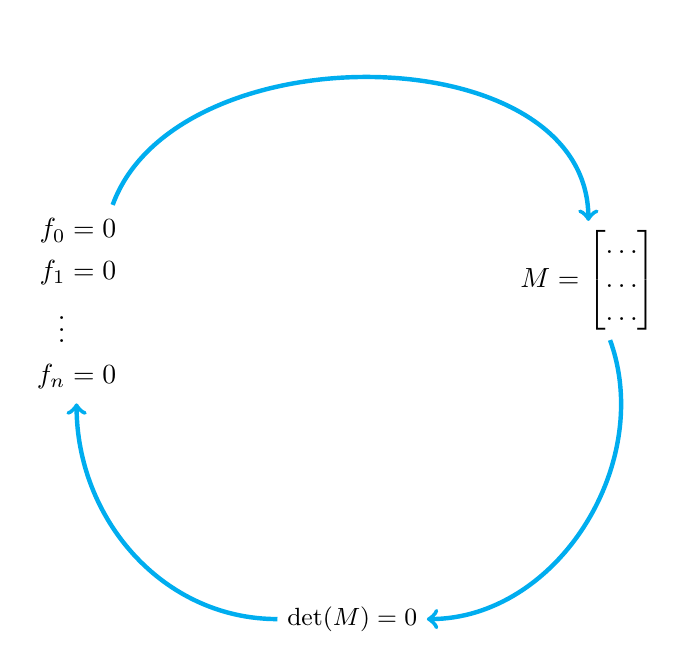
\begin{tikzpicture}
    
        \node (0) at (-0.5, 0) {$\begin{aligned}
            f_0 & = 0 \\
            f_1 & = 0 \\
            \vdots \\
            f_n & = 0
             \end{aligned}$};

        \node(1) at (6, 0.3) {$ M = \begin{bmatrix}
            \dots \\
            \dots \\
            \dots
          \end{bmatrix}$};
        \draw (0) edge[out=70, in=90, ->, ultra thick, cyan] node [above] {} (1);

        \node(2) at (3, -4) {\small{det$(M)= 0$}};
        \draw (1) edge[out=-70, in=0, ->, ultra thick, cyan] node [above] {} (2);
        \draw (2) edge[out=180, in=-90, ->, ultra thick, cyan] node [above] {} (0);
        \end{tikzpicture}
    
    \end{document}